\section{Números de Precisão Finita}
\title{Aula 6 - Precisão Finita (parte 3)}
\begin{frame}
    \titlepage
\end{frame}

\section{Números Fracionários}

\begin{frame}{Notação Posicional Fracionária}
    A representação de números fracionários expande a notação posicional para a direita do separador decimal, utilizando potências negativas da base $B$.

    $$(\sum_{i=0}^{m} b_i B^i) + (\sum_{j=-n}^{-1} b_j B^j)$$

    \begin{block}{Estrutura de Pesos}
        \centering
        \small
        \begin{tabular}{|c|c|c|c|c|c|c|}
            \hline
            $2^2$ & $2^1$ & $2^0$ & . & $2^{-1}$ & $2^{-2}$ & $2^{-3}$ \\ \hline
            4     & 2     & 1     & . & 0,5      & 0,25     & 0,125    \\ \hline
        \end{tabular}
    \end{block}

    \begin{exampleblock}{Exemplo: Binário $\rightarrow$ Decimal}
        $10100.011_2 = (16+4) + (0,25 + 0,125) = 20,375$
    \end{exampleblock}
\end{frame}

\begin{frame}{Conversão Decimal $\rightarrow$ Binário}
    Para converter um número fracionário da base 10 para a base 2:
    \begin{enumerate}
        \item Converta a \textbf{parte inteira} normalmente (divisões sucessivas).
        \item Use o algoritmo de \textbf{multiplicações sucessivas} para a parte fracionária ($n$).
    \end{enumerate}

    \begin{alertblock}{Algoritmo de Multiplicação}
        \begin{enumerate}
            \item Multiplique $n$ por 2.
            \item A parte inteira do resultado (0 ou 1) é o próximo bit.
            \item A nova parte fracionária vira o novo $n$.
            \item Repita até $n=0$ ou atingir a precisão desejada.
        \end{enumerate}
    \end{alertblock}
\end{frame}

\begin{frame}{Exemplo: Conversão de $20,375$}
    Parte inteira: $20_{10} = 10100_2$. Parte fracionária: $0,375$

    \begin{itemize}
        \item $0,375 \times 2 = \mathbf{0},75 \rightarrow b_{-1} = 0$
        \item $0,75 \times 2 = \mathbf{1},5 \rightarrow b_{-2} = 1$
        \item $0,5 \times 2 = \mathbf{1},0 \rightarrow b_{-3} = 1$ (Fim, pois $n=0$)
    \end{itemize}

    \begin{center}
        \textbf{Resultado:} $10100,011_2$
    \end{center}


\end{frame}

\begin{frame}{O Problema da Dízima Binária}
    Nem todo número decimal exato possui uma representação binária exata.

    \begin{exampleblock}{Exemplo: $20,3$}
        \begin{itemize}
            \item $0,3 \times 2 = 0,6 \rightarrow 0$
            \item $0,6 \times 2 = 1,2 \rightarrow 1$
            \item $0,2 \times 2 = 0,4 \rightarrow 0$
            \item $0,4 \times 2 = 0,8 \rightarrow 0$
            \item $0,8 \times 2 = 1,6 \rightarrow 1$
            \item $0,6 \times 2 = 1,2 \rightarrow 1$ (Ciclo iniciado!)
        \end{itemize}
    \end{exampleblock}

\end{frame}

\begin{frame}{Exercícios}
    Converta os seguintes números da base 10 para a base 2:

    \begin{enumerate}[a)]
        \item $20,5$
        \item $7,25$
        \item $0,625$
        \item $1,1$
    \end{enumerate}
\end{frame}
\begin{frame}{Gabarito: Conversão Fracionária}
    \tiny
    \begin{itemize}
        \item[\textbf{a)}] \textbf{20,5}:
              \begin{itemize}
                  \item Parte inteira: $20 = 10100_2$
                  \item Parte fracionária: $0,5 \times 2 = \mathbf{1},0$
                  \item \textbf{Resultado:} $10100,1_2$
              \end{itemize}

        \item[\textbf{b)}] \textbf{7,25}:
              \begin{itemize}
                  \item Parte inteira: $7 = 111_2$
                  \item Parte fracionária: $0,25 \times 2 = \mathbf{0},5 \rightarrow 0,5 \times 2 = \mathbf{1},0$
                  \item \textbf{Resultado:} $111,01_2$
              \end{itemize}

        \item[\textbf{c)}] \textbf{0,625}:
              \begin{itemize}
                  \item Parte inteira: $0 = 0_2$
                  \item Parte fracionária: $0,625 \times 2 = \mathbf{1},25 \rightarrow 0,25 \times 2 = \mathbf{0},5 \rightarrow 0,5 \times 2 = \mathbf{1},0$
                  \item \textbf{Resultado:} $0,101_2$
              \end{itemize}

        \item[\textbf{d)}] \textbf{1,1}:
              \begin{itemize}
                  \item Parte inteira: $1 = 1_2$
                  \item Parte fracionária: $0,1 \times 2 = \mathbf{0},2 \rightarrow 0,2 \times 2 = \mathbf{0},4 \rightarrow 0,4 \times 2 = \mathbf{0},8 \rightarrow 0,8 \times 2 = \mathbf{1},6 \rightarrow 0,6 \times 2 = \mathbf{1},2 \dots$
                  \item \textbf{Resultado:} $1,00011(0011)\dots_2$ (Dízima periódica)
              \end{itemize}
    \end{itemize}
\end{frame}

\section{Padrão IEEE 754}

\begin{frame}{O Padrão IEEE 754}
    O objetivo deste padrão é a interoperabilidade: garantir que um número fracionário gerado em um sistema seja interpretado da mesma forma em qualquer outro.

    \begin{itemize}
        \item \textbf{Categorias de Números:} Define representações para números normalizados, não normalizados e valores especiais.
        \item \textbf{Valores Especiais:}
              \begin{itemize}
                  \item Zero ($+0$ e $-0$)
                  \item Infinito ($\infty$ e $-\infty$)
                  \item \textbf{NaN} (\textit{Not a Number}): Resultados de operações inválidas (ex: $0/0$).
              \end{itemize}
        \item \textbf{Formatos Comuns:}
              \begin{itemize}
                  \item \textbf{Precisão Simples (\textit{float}):} 32 bits.
                  \item \textbf{Precisão Dupla (\textit{double}):} 64 bits.
              \end{itemize}
    \end{itemize}
\end{frame}

\begin{frame}{Notação Científica Binária}
    A base do padrão é a normalização do número binário, similar à notação científica decimal ($1,2 \times 10^3$). No binário, qualquer número (exceto o zero) pode ser escrito como:

    \[ \pm 1,xxxxx_2 \times 2^{yyyy} \]

    \begin{block}{Componentes da Representação}
        \begin{itemize}
            \item \textbf{Sinal ($S$):} Indica se o número é positivo ou negativo.
            \item \textbf{Mantissa ou Significando ($M$):} A parte fracionária ($xxxxx$).
                  \begin{itemize}
                      \item \textit{Nota: O "1" antes da vírgula é implícito (bit oculto) para economizar espaço.}
                  \end{itemize}
            \item \textbf{Expoente ($E$):} O valor da potência de 2 ($yyyy$).
        \end{itemize}
    \end{block}
\end{frame}

\subsection{IEEE 754: Precisão Simples (float)}

\begin{frame}{Layout da Precisão Simples (32 bits)}
    A representação de 32 bits é dividida em três campos específicos:

    \begin{itemize}
        \item \textbf{Sinal (S):} 1 bit (índice 31).
        \item \textbf{Expoente ($exp$):} 8 bits (índices 30 a 23).
        \item \textbf{Mantissa ($frac$):} 23 bits (índices 22 a 0).
    \end{itemize}

    \begin{block}{Arrumação dos Bits}
        \centering
        \texttt{\textbf{\color{red}S} \color{blue}EEEEEEEE \color{orange}MMMMMMMMMMMMMMMMMMMMMMM}
    \end{block}

    \begin{alertblock}{Dica de Leitura}
        Como 32 bits são difíceis de ler, agrupamos de 4 em 4 e representamos como \textbf{8 dígitos hexadecimais}.
    \end{alertblock}
\end{frame}

\begin{frame}{O Expoente}
    O expoente real ($E$) não é armazenado diretamente em Complemento a 2. Usa-se um \textbf{a lógica do excesso} de $127$.

    \begin{center}
        \Large $exp = E + 127$
    \end{center}

    \begin{itemize}
        \item \textbf{Faixa do Expoente Real ($E$):} $-126$ a $+127$.
        \item \textbf{Faixa no Campo ($exp$):} $1$ a $254$.
    \end{itemize}

    \begin{table}[]
        \begin{tabular}{l|l|l}
            \textbf{Significado} & \textbf{Expoente Real ($E$)} & \textbf{Valor em Bits ($exp$)} \\ \hline
            Menor valor          & $-126$                       & $00000001_2$ ($1$)             \\
            Zero real            & $0$                          & $01111111_2$ ($127$)           \\
            Maior valor          & $127$                        & $11111110_2$ ($254$)           \\
        \end{tabular}
    \end{table}
    \textit{*As combinações $00000000$ e $11111111$ são reservadas para casos especiais (Zero, NaN, Infinito).}
\end{frame}

\begin{frame}{A Mantissa e o Bit Oculto}
    Na notação normalizada, o número sempre começa com $1.xxxxx_2$.

    \begin{block}{Economia de Bits}
        Como o "$1$" antes da vírgula é sempre fixo para números normalizados, o padrão IEEE 754 \textbf{não o armazena}.
        Guardamos apenas a parte fracionária nos 23 bits.
    \end{block}



    \textbf{Pesos da Mantissa ($frac$):}
    Os bits da esquerda para a direita representam potências negativas:
    \begin{center}
        $2^{-1}, 2^{-2}, 2^{-3}, \dots, 2^{-23}$
    \end{center}
\end{frame}

\begin{frame}{Exemplo: Decodificando o Expoente}
    Se o campo de expoente na memória for \texttt{11110000}:

    \begin{enumerate}
        \item \textbf{Converter para Decimal ($exp$):}
              $11110000_2 = 128 + 64 + 32 + 16 = \mathbf{240}$

        \item \textbf{Subtrair o Viés (127):}
              $E = exp - 127$
              $E = 240 - 127 = \mathbf{113}$
    \end{enumerate}

    O número real está sendo multiplicado por $2^{113}$.
\end{frame}

\begin{frame}{Exemplo 1: Decodificação do Menor Expoente}
    Imagine que os 8 bits de expoente em uma representação IEEE 754 (Precisão Simples) sejam \texttt{00000001}.

    \begin{exampleblock}{Passo 1: Decodificar o campo $exp$ (Sem sinal)}
        $$exp = 00000001_2 = 2^0 = 1$$
    \end{exampleblock}

    \begin{exampleblock}{Passo 2: Calcular o expoente real $E$}
        Utilizando a lógica do excesso de 127 ($exp = E + 127$):
        $$E = exp - 127$$
        $$E = 1 - 127 = \mathbf{-126}$$
    \end{exampleblock}

    \textit{Este é o menor expoente real possível de ser representado em precisão simples para números normalizados.}
\end{frame}

\begin{frame}{Exemplo 2: Decodificação de Expoente Intermediário}
    Imagine agora que os 8 bits do campo de expoente sejam \texttt{11110000}.

    \begin{exampleblock}{Passo 1: Decodificar o campo $exp$}
        $$exp = 11110000_2 = 2^7 + 2^6 + 2^5 + 2^4$$
        $$exp = 128 + 64 + 32 + 16 = \mathbf{240}$$
    \end{exampleblock}

    \begin{exampleblock}{Passo 2: Calcular o expoente real $E$}
        $$E = exp - 127$$
        $$E = 240 - 127 = \mathbf{113}$$
    \end{exampleblock}

    Portanto, a potência de base 2 que multiplica a mantissa neste caso é $2^{113}$.
\end{frame}

\begin{frame}{Exemplo 3: Codificação do Maior Expoente}
    Agora queremos representar o maior expoente real possível em precisão simples: $E = 127$. Como codificar isso nos bits 30 a 23?

    \begin{exampleblock}{Passo 1: Obter o valor do campo $exp$ (Soma do excesso)}
        $$exp = E + 127$$
        $$exp = 127 + 127 = \mathbf{254}$$
    \end{exampleblock}

    \begin{exampleblock}{Passo 2: Converter $exp$ para binário (8 bits)}
        Convertendo $254$ para a base 2 (sem sinal):
        $$254 = 11111110_2$$
    \end{exampleblock}

    \vspace{0.3cm}
    Esta é a sequência de bits que deve ser inserida no campo de expoente para representar $E = 127$.
\end{frame}

%\begin{frame}{Visualizacao circular Complemento a 2}
%    \begin{center}
%        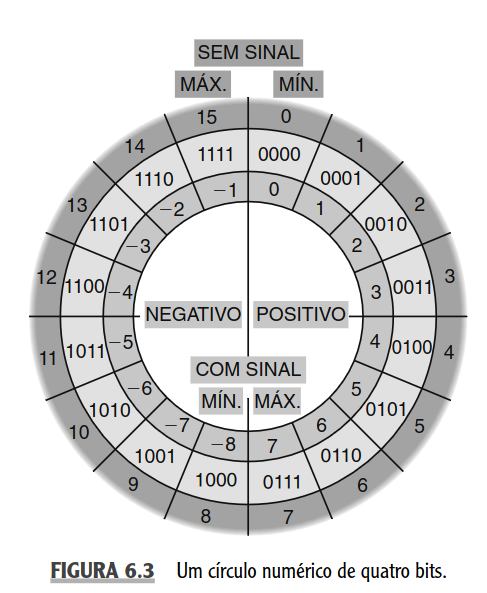
\includegraphics[width=0.5\textwidth]{Figuras/circulo-comp-a-2.png}
%    \end{center}
%\end{frame}